\documentclass[10pt]{article}

% Les figures sont copiées, et modifiées ou non du manuel de secondes de Sésamaths
% http://manuel.sesamath.net/

\usepackage{pablo}
\usepackage[a5paper,margin=1cm]{geometry}

\newcommand{\tikzcube}[1]{
    \begin{center}
      \begin{tikzpicture}[scale=#1,line width=1pt]
        \coordinate (O) at (0,0);
        \coordinate (x) at (1,0);
        \coordinate (y) at ({0.8*cos(30)},{0.8*sin(30)});
        \coordinate (z) at (0,1);

        \coordinate (A) at (O);
        \coordinate (B) at ($(O) + (x)$);
        \coordinate (C) at ($(O) + (x) + (y)$);
        \coordinate (D) at ($(O) + (y)$);
        \coordinate (E) at ($(O) + (z)$);
        \coordinate (F) at ($(O) + (z) + (x)$);
        \coordinate (G) at ($(O) + (z) + (x) + (y)$);
        \coordinate (H) at ($(O) + (z) + (y)$);

        \draw (A) node[below left]{$A$};
        \draw (B) node[below right]{$B$};
        \draw (C) node[right]{$C$};
        \draw (D) node[below]{$D$};
        \draw (E) node[left]{$E$};
        \draw (F) node[below right]{$F$};
        \draw (G) node[right]{$G$};
        \draw (H) node[above]{$H$};
        \draw (A) -- (B) -- (C) -- (G) -- (H) -- (E) -- (F) -- (B);
        \draw (A) -- (E);
        \draw (F) -- (G);
        \draw[dashed] (D) -- (H);
        \draw[dashed] (D) -- (A);
        \draw[dashed] (D) -- (C);

      \end{tikzpicture}
    \end{center}
}

\definecolor{A1}{cmyk}{1.00, 0.00, 0.00, 0.50}
\definecolor{A2}{cmyk}{0.60, 0.00, 0.00, 0.10}
\definecolor{A3}{cmyk}{0.30, 0.00, 0.00, 0.05}
\definecolor{A4}{cmyk}{0.10, 0.00, 0.00, 0.00}
\definecolor{B1}{cmyk}{0.00, 1.00, 0.60, 0.40}
\definecolor{B2}{cmyk}{0.00, 0.85, 0.60, 0.15}
\definecolor{B3}{cmyk}{0.00, 0.20, 0.15, 0.05}
\definecolor{B4}{cmyk}{0.00, 0.05, 0.05, 0.00}
\definecolor{C1}{cmyk}{0.00, 1.00, 0.00, 0.50}
\definecolor{C2}{cmyk}{0.00, 0.60, 0.00, 0.20}
\definecolor{C3}{cmyk}{0.00, 0.30, 0.00, 0.05}
\definecolor{C4}{cmyk}{0.00, 0.10, 0.00, 0.05}
\definecolor{D1}{cmyk}{0.00, 0.00, 1.00, 0.50}
\definecolor{D2}{cmyk}{0.20, 0.20, 0.80, 0.00}
\definecolor{D3}{cmyk}{0.00, 0.00, 0.20, 0.10}
\definecolor{D4}{cmyk}{0.00, 0.00, 0.20, 0.05}
\definecolor{F1}{cmyk}{0.00, 0.80, 0.50, 0.00}
\definecolor{F2}{cmyk}{0.00, 0.40, 0.30, 0.00}
\definecolor{F3}{cmyk}{0.00, 0.15, 0.10, 0.00}
\definecolor{F4}{cmyk}{0.00, 0.07, 0.05, 0.00}
\definecolor{G1}{cmyk}{1.00, 0.00, 0.50, 0.00}
\definecolor{G2}{cmyk}{0.50, 0.00, 0.20, 0.00}
\definecolor{G3}{cmyk}{0.20, 0.00, 0.10, 0.00}
\definecolor{G4}{cmyk}{0.10, 0.00, 0.05, 0.00}
\definecolor{H1}{cmyk}{0.40, 0.00, 1.00, 0.10}
\definecolor{H2}{cmyk}{0.20, 0.00, 0.50, 0.05}
\definecolor{H3}{cmyk}{0.10, 0.00, 0.20, 0.00}
\definecolor{H4}{cmyk}{0.07, 0.00, 0.15, 0.00}
\definecolor{J1}{cmyk}{0.00, 0.50, 1.00, 0.00}
\definecolor{J2}{cmyk}{0.00, 0.20, 0.50, 0.00}
\definecolor{J3}{cmyk}{0.00, 0.10, 0.20, 0.00}
\definecolor{J4}{cmyk}{0.00, 0.07, 0.15, 0.00}

\pagestyle{empty}

\begin{document}


\section{Droites et plans}

\begin{propriete}~
  \begin{itemize}
    \item Par deux points distincts $A$ et $B$ de l'espace passe \blanc{une unique droite}, notée \blanc{$(AB)$}.
    \item Par trois points $A$, $B$ $C$ non alignés de l'espace passe \blanc{un unique plan}, noté \blanc{$(ABC)$}.
    \item Si un plan contient deux points $A$ et $B$ distincts, alors il contient \blanc{tous les points} de la droite $(AB)$.
  \end{itemize}
\end{propriete}

\begin{propriete}
  Un plan peut être caractérisé par :
  \begin{itemize}
    \item \blanc{trois} points deux à deux distincts ;
    \item \blanc{une droite} et un point n'appartenant pas à cette droite ;
    \item \blanc{deux} droites sécantes ;
    \item \blanc{deux} droites strictement parallèles.
  \end{itemize}
\end{propriete}

\begin{definition}~
  \begin{itemize}
    \item Deux droites sont dites \blanc{coplanaires} s'il existe un plan qui les contient toutes les deux.
    \item Quatre points sont dits \blanc{coplanaires} s'il existe un plan qui les contient tous.
  \end{itemize}
\end{definition}

\begin{exemple}[On considère le cube $ABCDEFGH$, représenté ci-dessous.]~
  \begin{multicols}{2}
    \begin{enumerate}
      \item La droite $(FG)$ appartient aux plans \blanc{$(FGC)$} et \blanc{$(FGH)$}.
      \item 
        \begin{enumerate}
          \item $(HG)$ et $(GC)$ sont/ne sont pas coplanaires.
          \item $(EF)$ et $(DC)$ sont/ne sont pas coplanaires.
          \item $(EF)$ et $(GC)$ sont/ne sont pas coplanaires.
        \end{enumerate}

    \tikzcube{2}
      \item Marquer de la même couleur les plans identiques :
        \begin{enumerate}
          \item Le plan $(ABC)$
          \item Le plan contenant les droites $(EF)$ et $(FG)$.
          \item Le plan contenant les droites $(EF)$ et $(FA)$.
          \item Le plan contenant les droites $(EA)$ et $(FB)$.
          \item Le plan contenant la droite $(AB)$ et le point $F$.
          \item Le plan contenant la droite $(EF)$ et le point $H$.
          \item Le plan contenant la droite $(FA)$ et le point $B$.
          \item Le plan $(EFH)$.
        \end{enumerate}
    \end{enumerate}
  \end{multicols}
\end{exemple}


\pagebreak

\begin{multicols}{2}
\section{Positions relatives}
  \begin{em}
    Les exemples se réfèrent à la figure ci-contre.
  \end{em}

  \tikzcube{2}
\end{multicols}

\begin{propriete}[Position relative d'une droite et d'un plan]
  Une droite et un plan peuvent être :

  \begin{center}
  \begin{tabular}{|p{.3\textwidth}|p{.3\textwidth}|p{.3\textwidth}|}
    \hline
    \multicolumn{1}{|c|}{Sécants} & \multicolumn{2}{c|}{Parallèles} \\
    & \multicolumn{1}{c|}{Strictement parallèles} & \multicolumn{1}{c|}{Confondus} \\
    \hline
    %Leur intersection est alors un point. & Ils n'ont alors aucun point d'intersection & La droite est incluse dans le plan \\
    &&\\[2cm]
    \hline
    Exemple : & Exemple : & Exemple : \\[2cm]
    &&\\
    \hline
  \end{tabular}
\end{center}
\end{propriete}


\begin{propriete}[Position relative de deux plans]
  Deux plans peuvent être :

  \begin{center}
  \begin{tabular}{|p{.3\textwidth}|p{.3\textwidth}|p{.3\textwidth}|}
    \hline
    \multicolumn{1}{|c|}{Sécants} & \multicolumn{2}{c|}{Parallèles} \\
    & \multicolumn{1}{c|}{Strictement parallèles} & \multicolumn{1}{c|}{Confondus} \\
    \hline
    %Leur intersection est alors une droite. & Ils n'ont alors aucun point d'intersection & \\
    &&\\[2cm]
    \hline
    Exemple : & Exemple : & Exemple : \\[2cm]
    &&\\
    \hline
  \end{tabular}
\end{center}
\end{propriete}

\pagebreak
\section{Paraléllisme entre droites et plans}
\emph{\noindent Indiquer à côté de chaque propriété ou théorème le numéro de la figure qui l'illustre. Une figure peut illustrer plusieurs propriétés.}

% Les figures sont copiées, et modifiées ou non du manuel de secondes de Sésamaths
% http://manuel.sesamath.net/
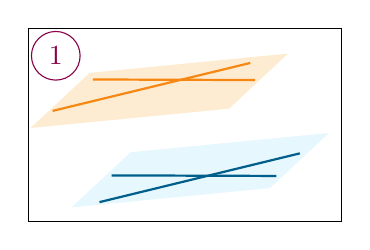
\begin{tikzpicture}[xscale=0.5,yscale=0.35]
  \draw (-1.1,-0.5) rectangle (6.86,6.5);
  \draw (-0.4,5.5) node[circle, draw, color=C1] { 1};
%plan du haut (Couleurs chaudes)
  \fill[color=J4,fill=J4] (0.46,4.88) -- (-1.04,2.88) -- (4,3.58) -- (5.5,5.58) -- cycle;
  \draw [thick,color=J1] (-0.48,3.5)-- (4.54,5.24);%droite "croissante"
  \draw [thick,color=J1] (0.54,4.64)-- (4.66,4.62);%droite "d´ecroissante"
%plan du bas (couleurs froides)
  \fill[color=A4,fill=A4] (1.5,2) -- (0,0) -- (5.04,0.7) -- (6.54,2.7) -- cycle;
  \draw [thick,color=A1] (1.02,1.16)-- (5.2,1.14);%droite "d´ecroissante"
  \draw [thick,color=A1] (5.8,1.96)-- (0.71,0.19);%droite "croissante"
\end{tikzpicture}
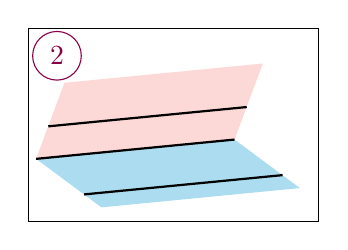
\begin{tikzpicture}[xscale=0.5,yscale=0.35]
  \draw(-1.86,-0.5) rectangle (5.52,6.5);
  \draw (-1.13,5.5) node[circle, draw, color=C1] { 2};
  \fill[color=A3,fill=A3] (-1.66,1.76) -- (0,0) -- (5.04,0.7) -- (3.38,2.46) -- cycle;  % plan du bas en couleur froide
  \fill[color=F3,fill=F3] (-1.66,1.76) -- (3.38,2.46) -- (4.1,5.22) -- (-0.94,4.52) -- cycle;  %plan du haut en couleur chaude
  \draw [thick] (-0.44,0.47)-- (4.6,1.17);%droite dans le plan du haut, en trait gras, en noir?
  \draw [thick] (-1.35,2.94)-- (3.69,3.64);%droite dans le plan du bas, en trait gras, en noir?
  \draw [thick] (-1.66,1.76)-- (3.38,2.46);%droite d'intersection des deux plans, en trait gras, en noir?
\end{tikzpicture}
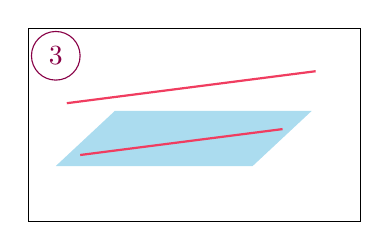
\begin{tikzpicture}[xscale=0.5,yscale=0.35]
  \draw (0,4) node[circle, draw, color=C1] { 3};
  \draw(-0.7,-2) rectangle (7.74,5);
  \fill[color=A3,fill=A3] (1.5,2) -- (0,0) -- (5,0) -- (6.5,2) -- cycle;
  \draw [thick,color=F1]  (5.76,1.34)-- (0.62,0.4);%droite du haut
  \draw [thick,color=F1] (0.28,2.28)-- (6.6,3.44);%droite dans le plan
\end{tikzpicture}

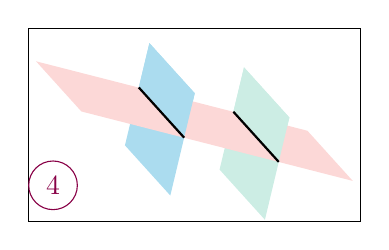
\begin{tikzpicture}[xscale=0.45,yscale=0.35]
  \draw(-3.92,-2.5) rectangle (5.46,4.5);
  \fill[color=A3,fill=A3] (-0.5,3.96) -- (-1.19,0.25) -- (0.09,-1.57) -- (0.78,2.14) -- cycle;  %plan "vertical" de gauche bas
  \fill[color=G3,fill=G3] (2.17,3.08) -- (1.48,-0.63) -- (2.76,-2.45) -- (3.45,1.26) -- cycle; %plan "vertical" de droite bas
  \fill[color=F3,fill=F3] (-3.7,3.3) -- (-2.42,1.48) -- (5.24,-1.04) -- (3.96,0.78) -- cycle; %plan "horizontal"
  \fill[color=A3,fill=A3] (-0.5,3.96) -- (0.78,2.14) -- (0.48,0.53)-- (-0.8,2.35) -- cycle;  %plan "vertical" de gauche haut
  \fill[color=G3,fill=G3] (2.17,3.08) -- (3.45,1.26) --  (3.15,-0.35) --(1.87,1.47)-- cycle; %plan "vertical" de droite haut
  \draw [thick] (0.48,0.53)-- (-0.8,2.35); %droite d'intersection de gauche
  \draw [thick] (1.87,1.47)-- (3.15,-0.35); %droite d'intersection de droite
  \draw (-3.22,-1.2) node[circle, draw, color=C1] { 4};
\end{tikzpicture}
\hspace{\stretch{1}}
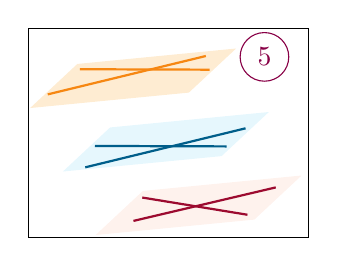
\begin{tikzpicture}[xscale=0.5,yscale=0.35]
  \begin{scope}[scale=.8]
  \draw (-1.1,-3.0) rectangle (7.8,6.5);
  \draw (6.4,5.2) node[circle, draw, color=C1] { 5};
%plan du haut (Couleurs chaudes)
  \fill[color=J4,fill=J4] (0.46,4.88) -- (-1.04,2.88) -- (4,3.58) -- (5.5,5.58) -- cycle;
  \draw [thick,color=J1] (-0.48,3.5)-- (4.54,5.24);%droite "croissante"
  \draw [thick,color=J1] (0.54,4.64)-- (4.66,4.62);%droite "d´ecroissante"
%plan du milieu (couleurs froides)
  \fill[color=A4,fill=A4] (1.5,2) -- (0,0) -- (5.04,0.7) -- (6.54,2.7) -- cycle;
  \draw [thick,color=A1] (1.02,1.16)-- (5.2,1.14);%droite "d´ecroissante"
  \draw [thick,color=A1] (5.8,1.96)-- (0.71,0.19);%droite "croissante"
%plan du bas (couleurs froides)
  \fill[color=B4,fill=B4] (2.54,-.88) -- (1.04,-2.88) -- (6.08,-2.18) -- (7.58,-0.18) -- cycle;
  \draw [thick,color=B1] (2.52,-1.18)-- (5.86,-1.96);%droite "d´ecroissante"
  \draw [thick,color=B1] (6.76,-0.72)-- (2.24,-2.24);%droite "croissante"
\end{scope}
\end{tikzpicture}
\hspace{\stretch{1}}
\begin{tikzpicture}[xscale=0.5,yscale=0.35]
  \draw (-1.3,1.5) rectangle (6.7,7.5);
  \draw (-0.4,6.3) node[circle, draw, color=C1] { 6};
  \begin{scope}[scale=1.1]
  \coordinate (A) at (0.52,5.8);
  \coordinate (B) at (2.2,2);
  \coordinate (C) at (2.02,6.3);
  \coordinate (D) at (3.7,2.3);
  \draw [thick,color=B1] ($(A)!.6!(B)$) -- (B);
  \draw [thick,color=B1] ($(C)!.6!(D)$) -- (D);
%plan du haut (Couleurs chaudes)
  \fill[color=J4,fill=J4] (0.46,4.88) -- (-1.04,2.88) -- (4,3.58) -- (5.5,5.58) -- cycle;
  \draw [thick, color=B1] (A) -- ($(A)!.4!(B)$);
  \draw [thick,dashed, color=B1] ($(A)!.4!(B)$) -- ($(A)!.6!(B)$);
  \draw [thick, color=B1] (C) -- ($(C)!.4!(D)$);
  \draw [thick,dashed, color=B1] ($(C)!.4!(D)$) -- ($(C)!.6!(D)$);
\end{scope}
\end{tikzpicture}

\begin{propriete}
  Si deux droites sont parallèles, toute droite parallèle à l'une est parallèle à l'autre.
\end{propriete}

\begin{propriete}
  Si deux droites sont parallèles, tout plan sécant avec l'une est sécant avec l'autre.
\end{propriete}

\begin{propriete}
  Une droite parallèle à une autre droite contenue dans un plan est parallèle à ce plan.
\end{propriete}

\begin{theoreme}[Théorème du toit]
  Soient $\mathcal{P}_1$ et $\mathcal{P}_2$ deux plans, et $d_1$ et $d_2$ deux droites, tels que :
  \begin{itemize}
    \item $d_1$ et $d_2$ sont parallèles ;
    \item $d_1$ est incluse dans $\mathcal{P}_1$ ;
    \item $d_2$ est incluse dans $\mathcal{P}_2$ ;
    \item $\mathcal{P}_1$ et $\mathcal{P}_2$ sont sécants selon une droite $\delta$.
  \end{itemize}
  Alors $d_1$ et $d_2$ sont parallèles à $\delta$.

\end{theoreme}

\begin{propriete}
  Si deux plans sont parallèles, tout plan sécant avec l'un est sécant avec
  l'autre, et les droites d'intersection sont parallèles.
\end{propriete}

\begin{propriete}
  Si deux plans sont parallèles, tout plan parallèle à l'un est parallèle à l'autre.
\end{propriete}

\begin{propriete}
  Si un plan $\mathcal P$ contient deux droites sécantes et parallèles à un
  plan $\mathcal P'$, alors les plans $\mathcal P$ et $\mathcal P'$ sont
  parallèles.
\end{propriete}


\end{document}
